\section{Basic Compensation}
\label{sec:basic}

The first compensation stage accounts for basic amplifier characteristics which make it not-linear.
Figure \ref{fig:iobasic} shows the amplifier output voltage (y axis) vs input voltage (x axis) for a resistive load.
Three characteristics of the curve should be noted.
First, it has a dead-zone where output voltage is zero for a range of input voltages.
Second, the input voltage which produces a zero output voltage is not zero.
Finally, in the linear regions, gain is not one.
A simple block diagram to compensate for these effects can be seen in figure \ref{fig:iobasiccomp} and the full Simulink block in figure \ref{fig:simulink}.

\begin{figure}[ht]
    \centering
    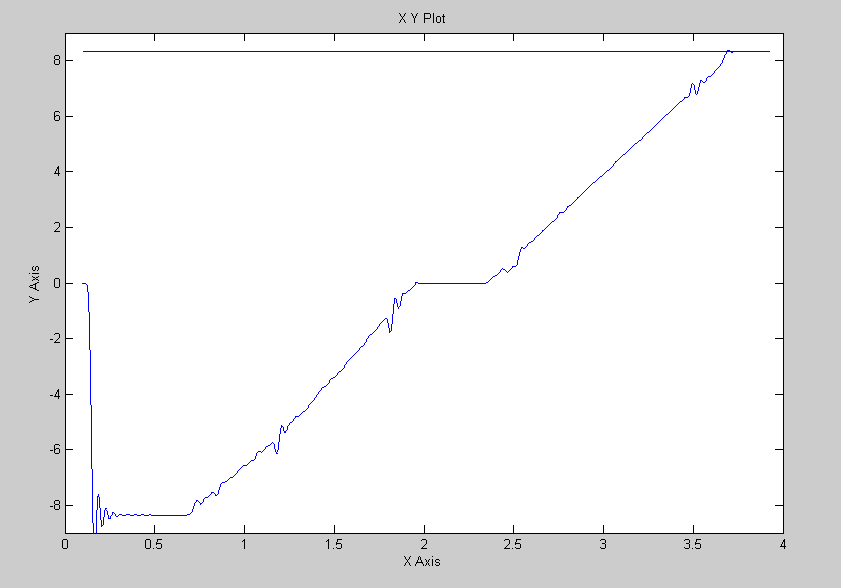
\includegraphics[width=.70\textwidth]{images/InputVsOutputResistive2.PNG}
    \caption{Amplifier Input Voltage vs Output Voltage for Resistive Load}
    \label{fig:iobasic}
\end{figure}

\begin{figure}[ht]
    \centering
    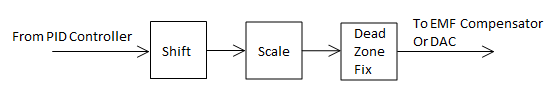
\includegraphics[width=.65\textwidth]{images/BasicCompensator.PNG}
    \caption{Basic Compensation Block Diagram}
    \label{fig:iobasiccomp}
\end{figure}

The input-output relationship when using these compensation steps may be seen in \ref{fig:iocomp}.
It can be seen that when using the compensator, the amplifier response (given a purely resistive load) is far more linear.
This compensation mechanism is dependent on accurately known the saturation and dead zone limits of the amplifier.
A simulink to block automatically calibrate parameters may be seen in \ref{fig:simulinkfinder}.

\begin{figure}[ht]
    \centering
    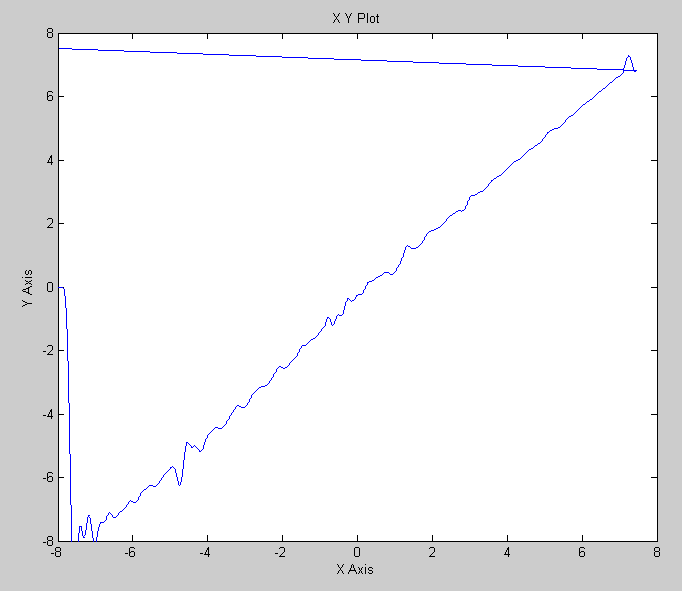
\includegraphics[width=.70\textwidth]{images/CompensatedOutput.PNG}
    \caption{Compensated Amplifier Input Voltage vs Output Voltage for Resistive Load}
    \label{fig:iocomp}
\end{figure}
